\chapter{Data Analysis II: Extracting Physics}

\section{Edge Cuts}
As seen in Fig.~\ref{fig:edge}, edges of the measurement volume of the TPC we can see several edge effects distortion the clusters positions. The last pads on the edges of the pad-plane naturally have no neighbors on the outsides, therefore their cluster position is biased towards the inside of the TPC. Also since we measure a finite window in time for the vertical direction, pulses near the edge of the time-bucket window are clipped and the reconstructed times are biased towards inside the TPC volume. 

The number of clusters affected is small but the deviation at the end of the track is enough to start causing issues in the momentum reconstruction. Simple cuts around the left,right, top, and bottom of the TPC remove these clusters from the analysis,

\begin{equation*}
  |x|\geq420~\mathrm{mm},\quad y\leq-522+\mathrm{y_o}~\mathrm{mm},
  \quad\mathrm{and}\quad y\geq-64+\mathrm{(Hit\ Shift)}~\mathrm{mm}.
  \label{eq:hitshift}
\end{equation*}

\begin{figure}[!htb]
    \centering
    \begin{subfigure}[t]{0.45\textwidth}
        \centering
        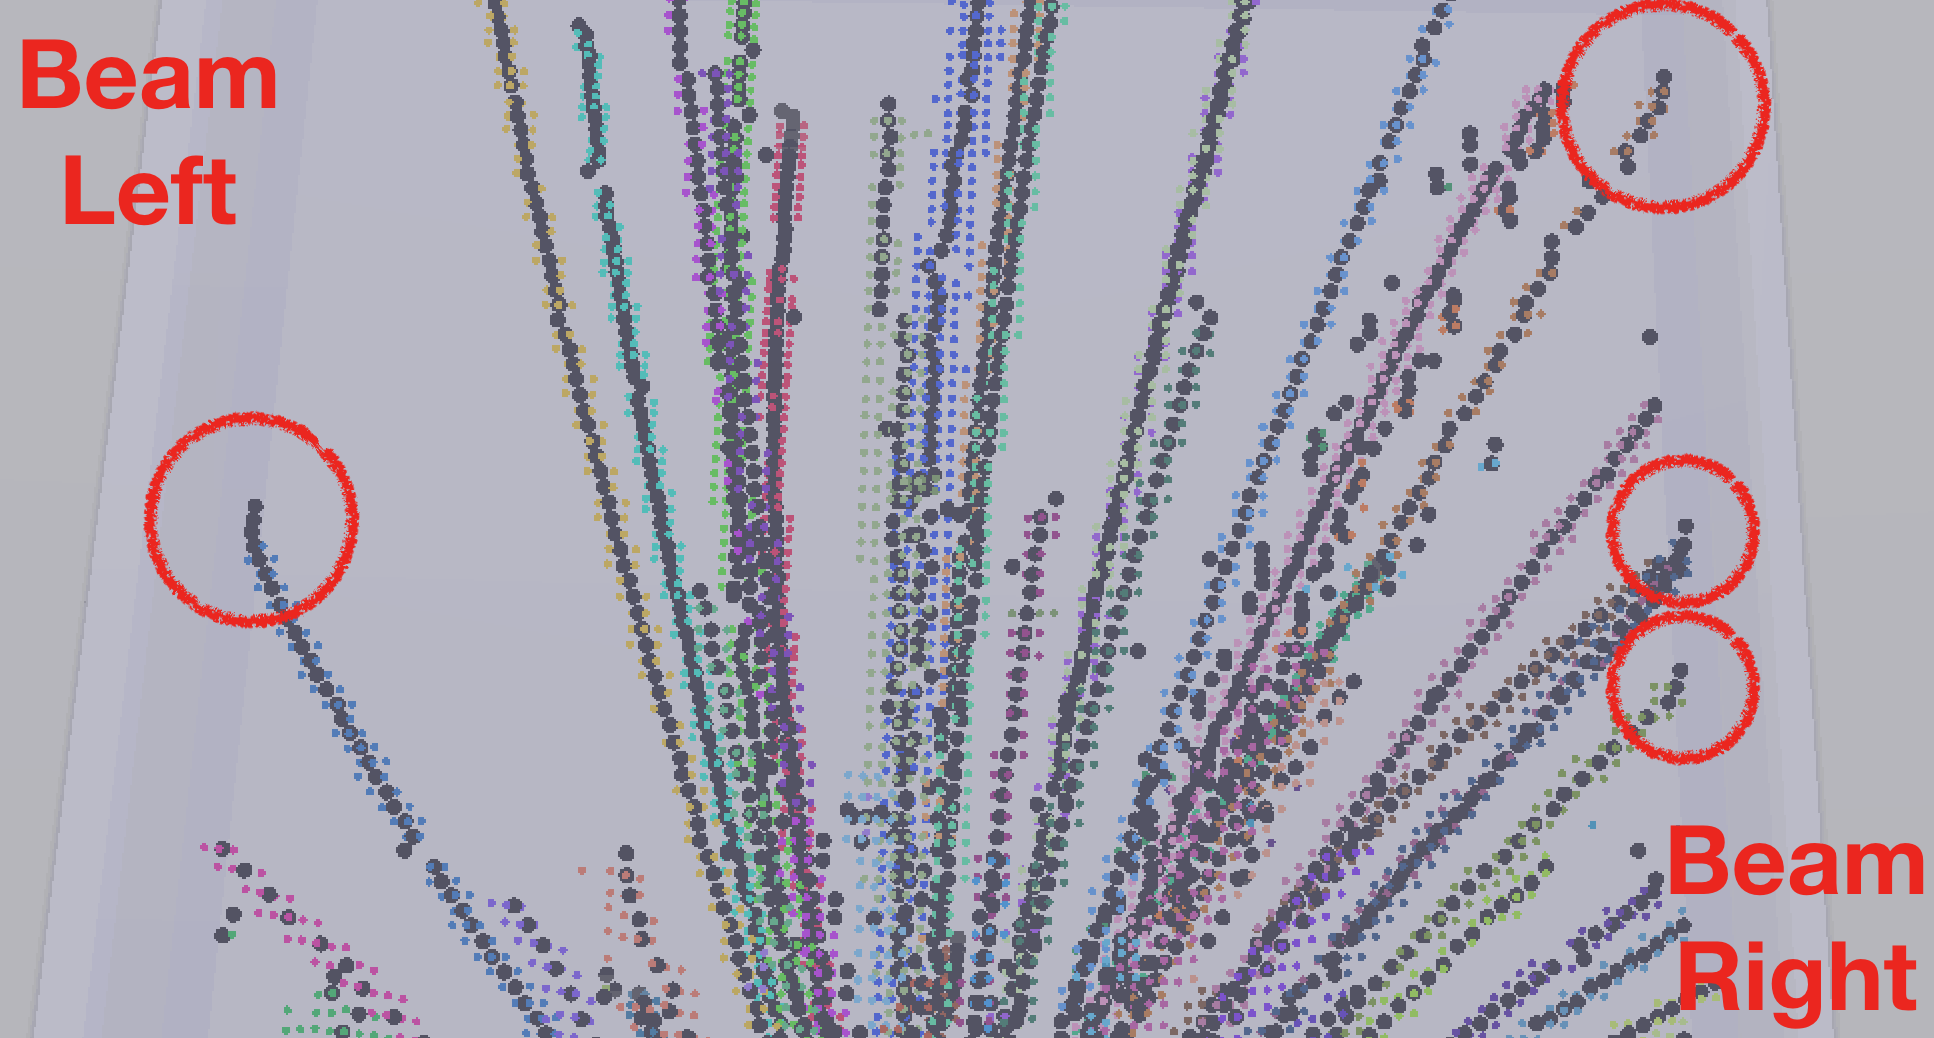
\includegraphics[width=\linewidth]{clusterLR.png} 
        \caption{Generic} \label{fig:mom_S_before}
    \end{subfigure}
    \hfill
    \begin{subfigure}[t]{0.45\textwidth}
        \centering
        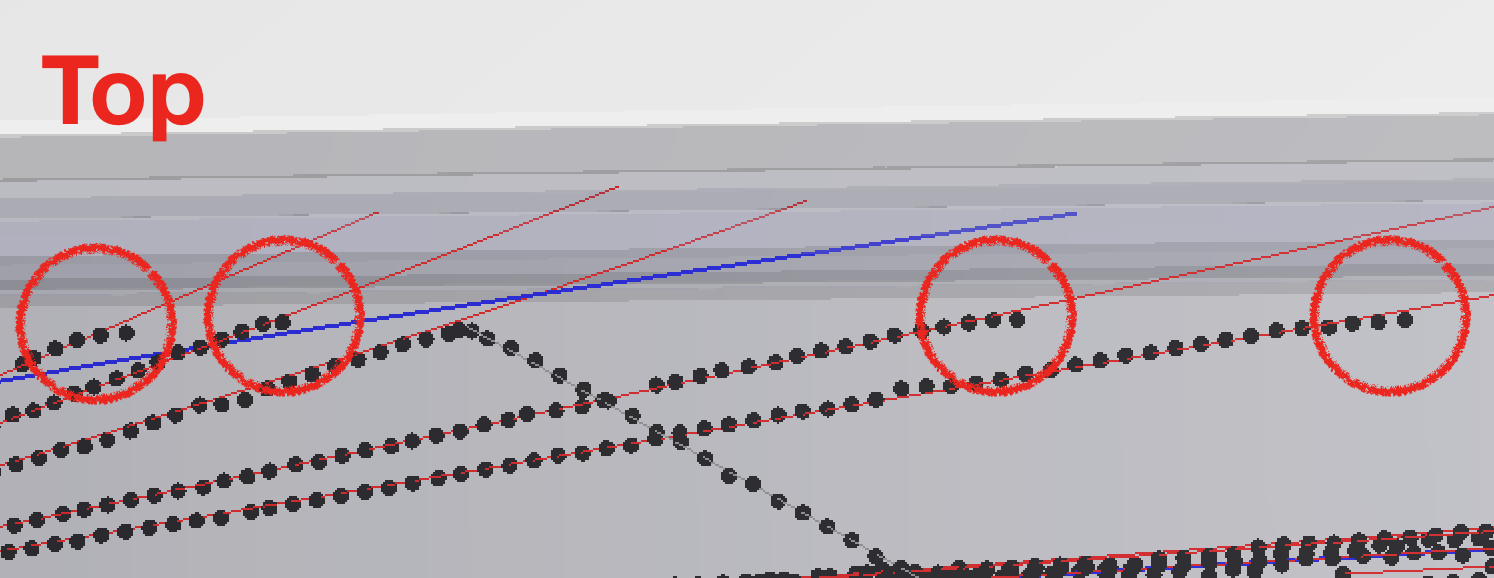
\includegraphics[width=\linewidth]{clusterTop.png} 
        \caption{Competitors} \label{fig:mom_L_before}
    \end{subfigure}
    
    \begin{subfigure}[t]{0.45\textwidth}
        \centering
        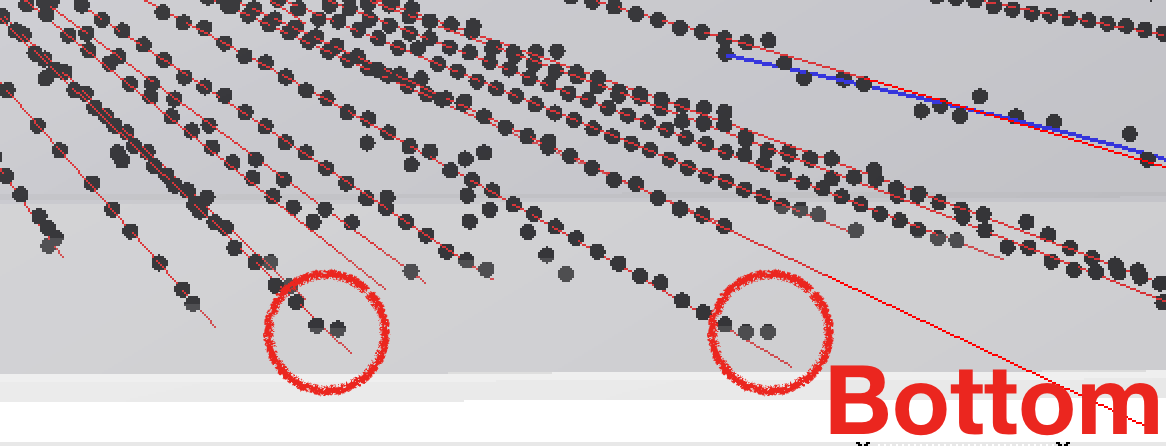
\includegraphics[width=\linewidth]{clusterBottom.png} 
        \caption{Generic} \label{fig:mom_S_after}
    \end{subfigure}
   
\label{fig:edge}
\end{figure}

\section{High Density Cut}
The density of tracks near the target region is very high and most of electronics information from this region is inaccurate in both timing and charge value. Hits lying within an semi-ellipsoidal cut region around the target are removed from the software and not included in the track and momentum reconstruction. 

Add picture of ellipsoid 

\section{Beam angle selection}
The beam is bent by the magnetic field before hitting the target. The BDCs track the beam outside of the magnet. The beam is then propagated through the magnetic field until the target position. The beam angle on target is categorized by two angles $\theta_{a,proj}$ and $\theta_

\begin{figure}[!htb]
    \centering
    \begin{subfigure}[t]{0.45\textwidth}
        \centering
        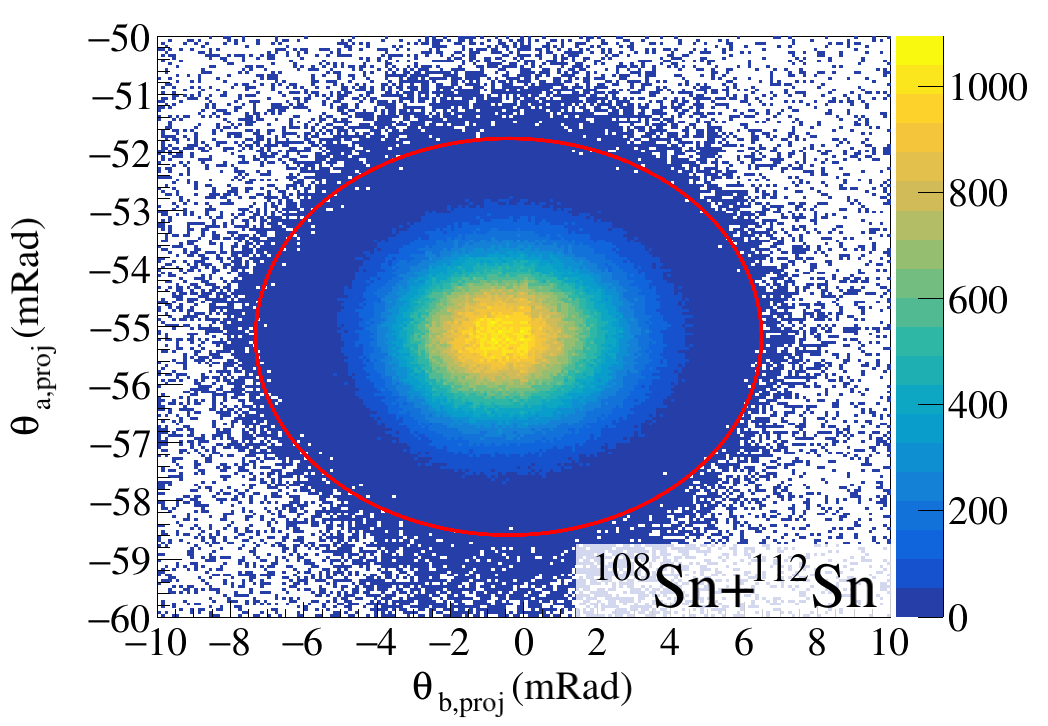
\includegraphics[width=\linewidth]{beamAngle-Sn108.png} 
        \caption{Generic} \label{fig:mom_S_before}
    \end{subfigure}
    \hfill
    \begin{subfigure}[t]{0.45\textwidth}
        \centering
        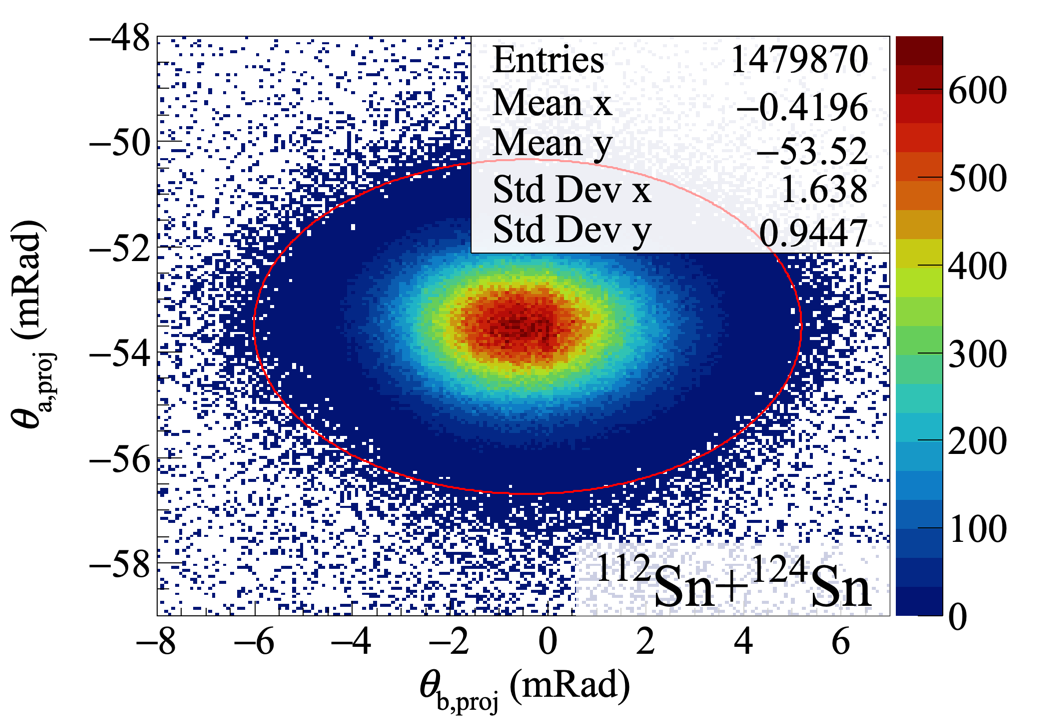
\includegraphics[width=\linewidth]{beamAngle-Sn112.png} 
        \caption{Competitors} \label{fig:mom_L_before}
    \end{subfigure}
    
    \begin{subfigure}[t]{0.45\textwidth}
        \centering
        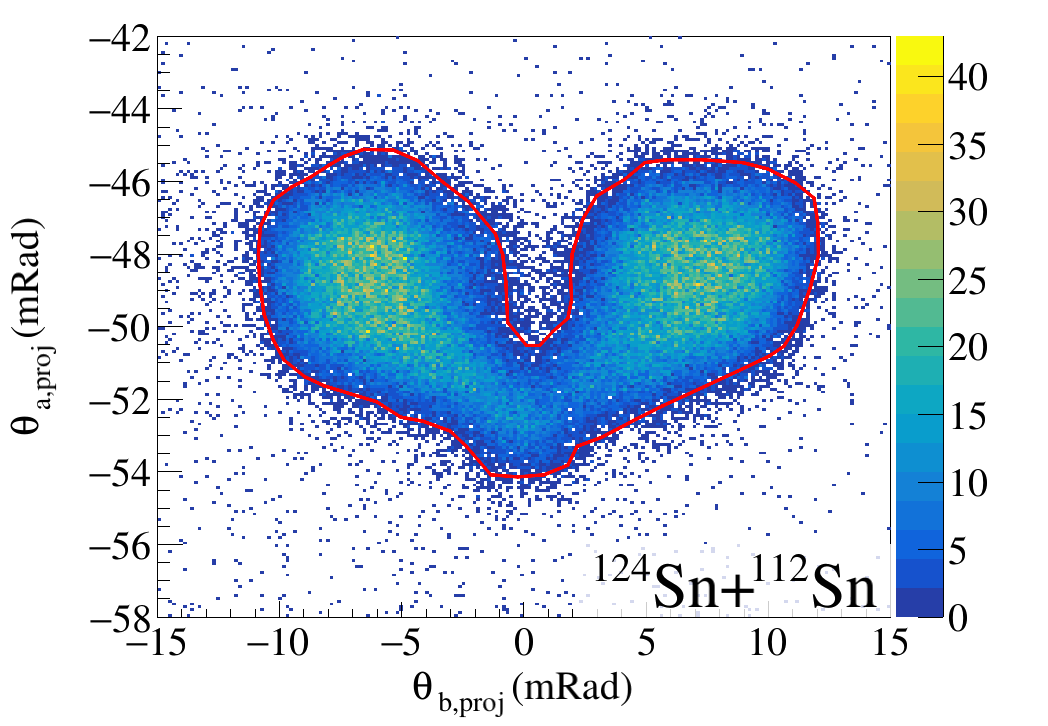
\includegraphics[width=\linewidth]{beamAngle-Sn124.png} 
        \caption{Generic} \label{fig:mom_S_after}
    \end{subfigure}
    \hfill
    \begin{subfigure}[t]{0.45\textwidth}
        \centering
        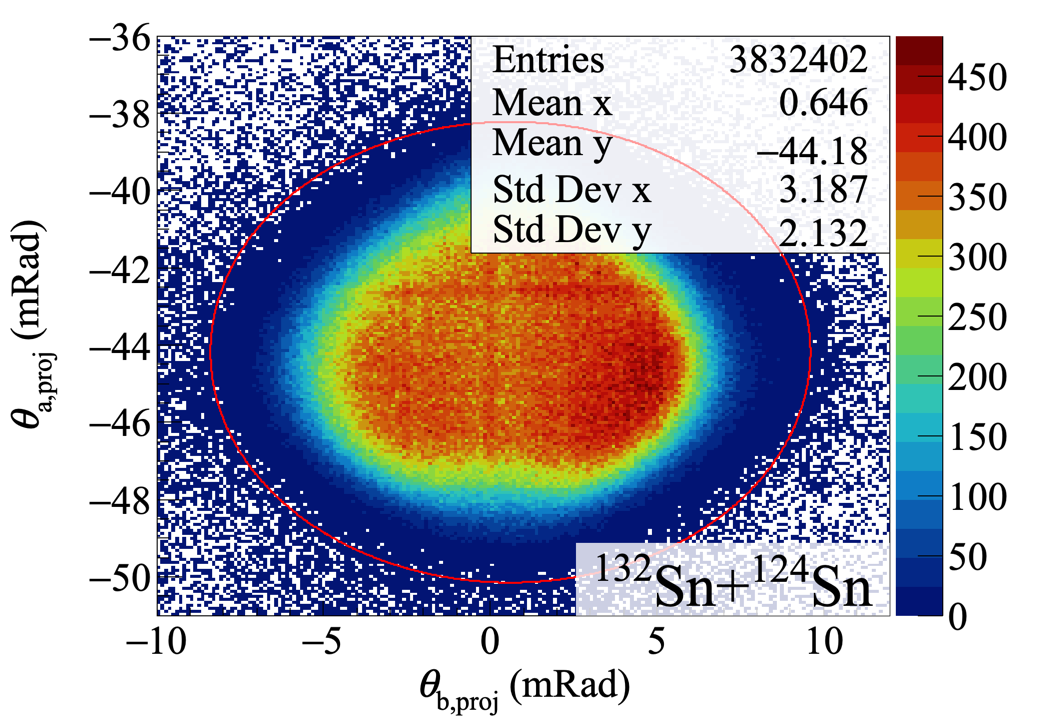
\includegraphics[width=\linewidth]{beamAngle-Sn132.png} 
        \caption{Competitors} \label{fig:mom_L_after}
    \end{subfigure}
\label{fig:mom_sc}
\end{figure}



\section{Vertex Cut}


\begin{figure}[!htb]
    \centering
    \begin{subfigure}[t]{\textwidth}
        \centering
        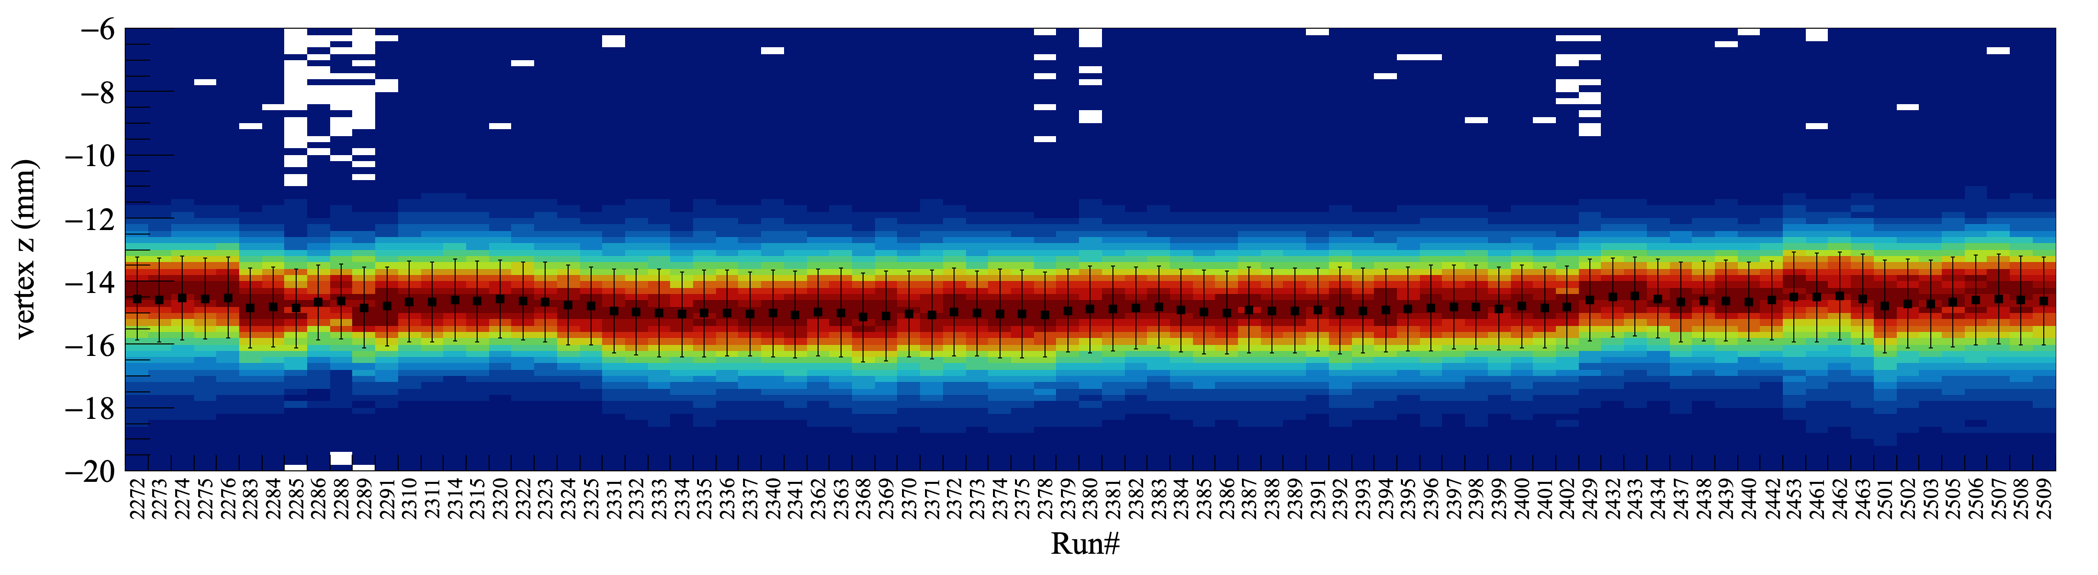
\includegraphics[width=\linewidth]{vertex-Sn108.png} 
        \caption{$\tin{108}{124}$ vertex distributon for all runs.} \label{fig:vertex108}
    \end{subfigure}
    \hfill
    \begin{subfigure}[t]{\textwidth}
        \centering
        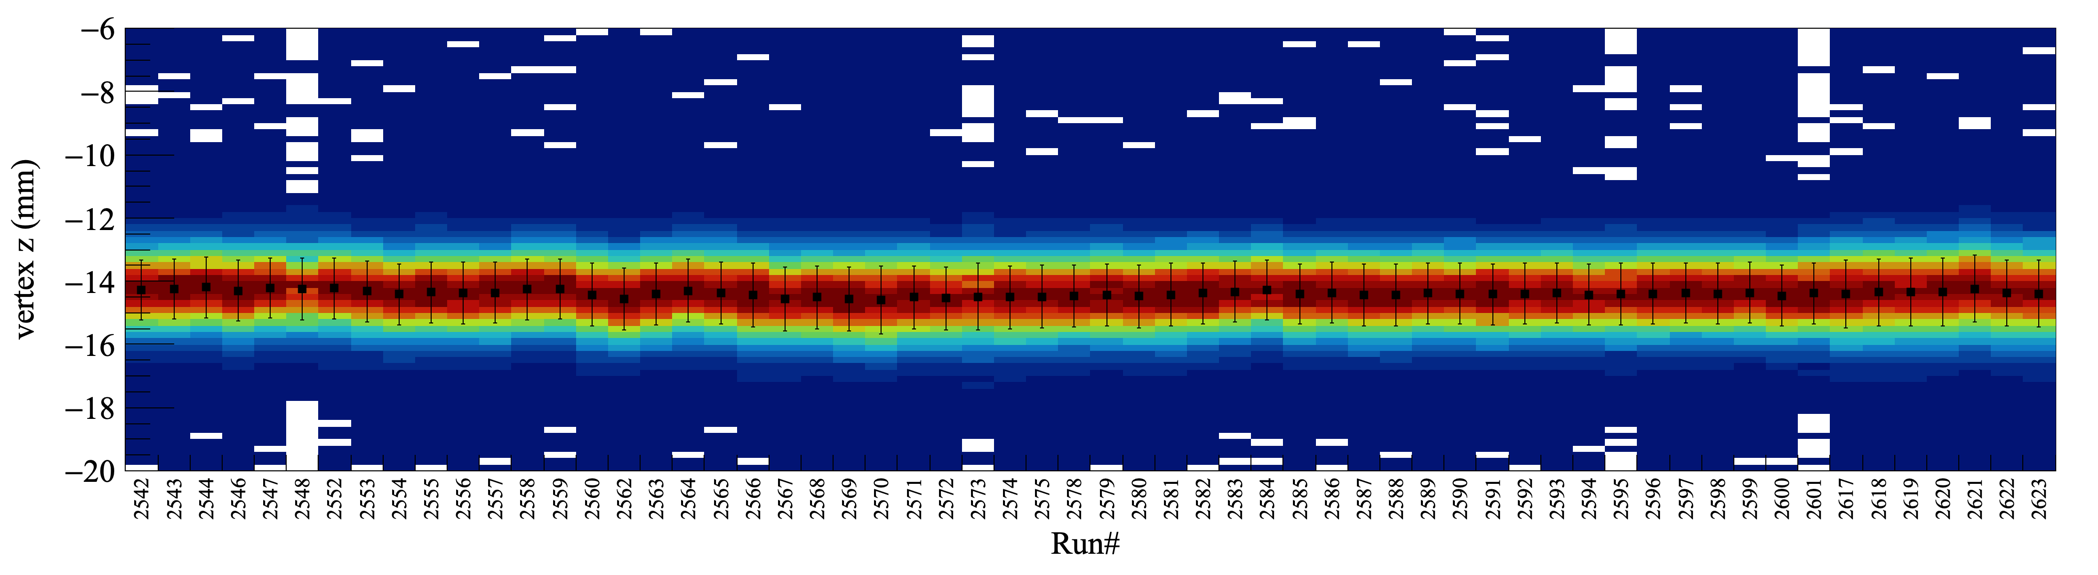
\includegraphics[width=\linewidth]{vertex-Sn112.png} 
        \caption{$\tin{112}{124}$ vertex distributon for all runs.} \label{fig:vertex112}
    \end{subfigure}
    
    \begin{subfigure}[t]{\textwidth}
        \centering
        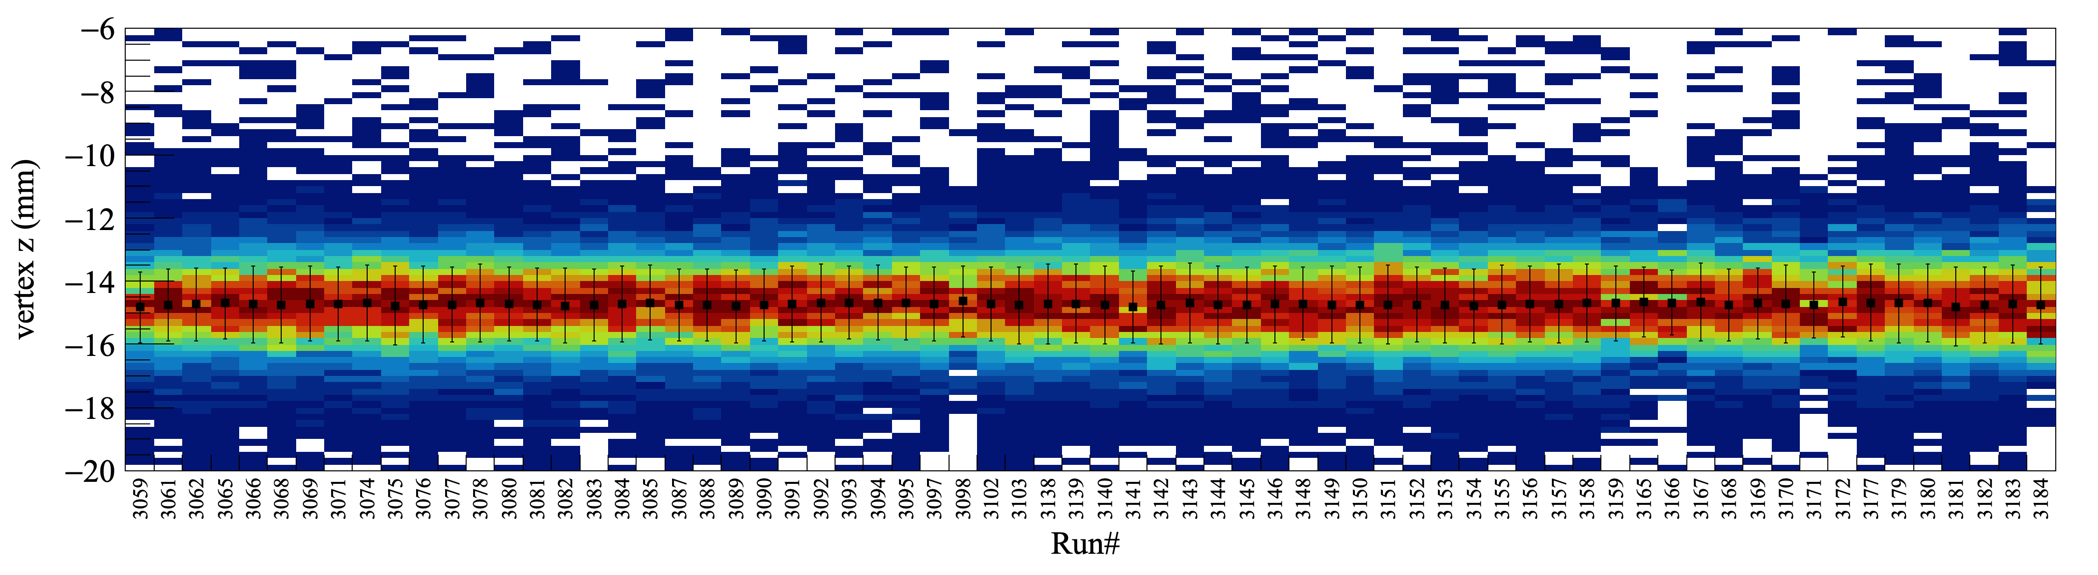
\includegraphics[width=\linewidth]{vertex-Sn124.png} 
        \caption{$\tin{124}{112}$ vertex distributon for all runs.} \label{fig:vertex124}
    \end{subfigure}
    \hfill
    \begin{subfigure}[t]{\textwidth}
        \centering
        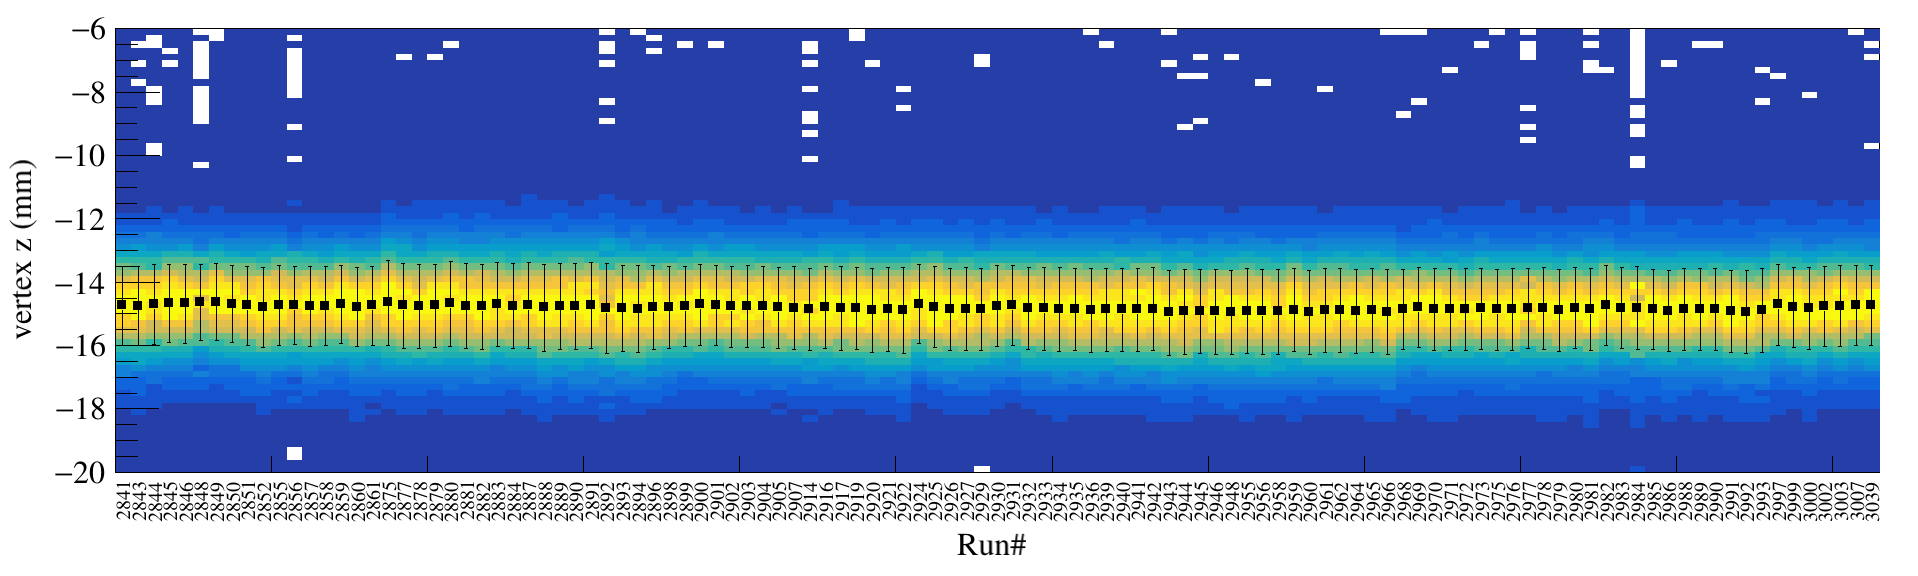
\includegraphics[width=\linewidth]{vertex-Sn132.png} 
        \caption{$\tin{132}{124}$ vertex distributon for all runs.} \label{fig:vertex132}
    \end{subfigure}
\label{fig:vertexdist}
\end{figure}


\section{Impact Parameter Selection}


\section{Track Quality Cuts}



\section{Angular Quality Cuts}

